\chapter{Testing and Results}

In order to examine the performance and robustness of my approach, a serious of experiments target both individual functions and the integrated system has been conducted. The success rate and execution times are the two evaluation criteria.

In all experiments, I utilize the same platform as shown in Figure \ref{5.1}. It consists of a YuMi robot and an external camera (ZED Mini or ASUS Xtion). In order to maximize the accuracy while ensuring a reasonable frame speed, ZED Mini camera with 1080p resolution is chosen for all the experiments in this chapter. The marked shoe will be placed on the workbench within the area YuMi can reach. All tests were conducted under normal lighting conditions. 

\section{Shoe Detection and Coordinate Estimation}
The purpose of this part experiment is to assess the robustness of object detection and if the system can correctly compute adjustment locations or the centroid of the shoe hole.

The marked shoe will be placed at random location on the workbench for 10 times, together with other disturbing objects. For each location, I rotate the shoe 5 times to adjust its orientation. YOLO algorithm will be used to perform shoe detection and return the prediction probability and the bounding box. Its performance is illustrated in Table \ref{yolotest}.

\begin{table}[H]
\centering
\resizebox{\columnwidth}{!}{
\begin{tabular}{||c||c|c|c|c|c|c||}
\hline
 & \begin{tabular}[c]{@{}c@{}}Average \\ execution time\end{tabular} & \begin{tabular}[c]{@{}c@{}}Success \\ rate\end{tabular} & \begin{tabular}[c]{@{}c@{}}Average\\ probability\end{tabular} & \begin{tabular}[c]{@{}c@{}}Minimum \\ probability\end{tabular} & \begin{tabular}[c]{@{}c@{}}Maximum \\ probability\end{tabular} & \begin{tabular}[c]{@{}l@{}}Standard \\ deviation\end{tabular} \\ \hline
 \hline
Shoe detection & 0.052s & 50/50 & 0.65 & 0.36 & 0.96 & 0.17 \\ \hline
\end{tabular}}
\caption{The testing results of YOLO shoe detection}
\label{yolotest}
\end{table}

As can be seen, the shoe detection system achieved 100\% success rate in these 50 tests with high detection speed. The relatively large fluctuation of detection probability is due to several low readings. These low probabilities are obtained when the shoe is placed on the edge of the image captured by the camera, such as Figure \ref{yolotestexample}. Overall, the performance of shoe detection is desirable. 

\begin{figure}[H]
\centering
\subfigure[Low confidence when the shoe is placed on the edge of the image]{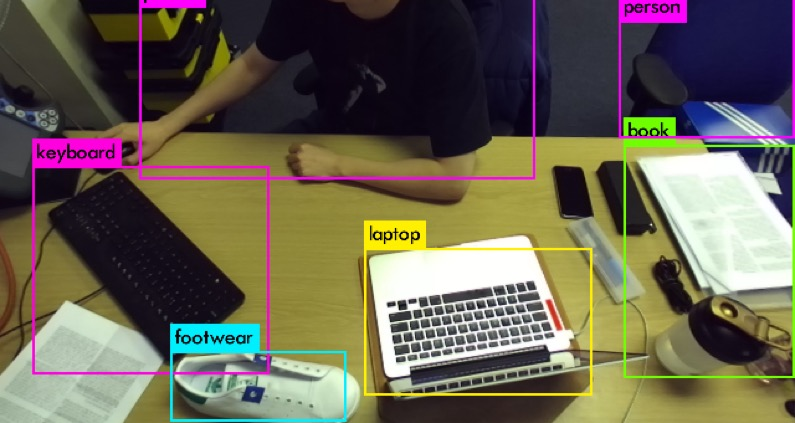
\includegraphics[width = 0.45\columnwidth]{TaR/yolot1.jpg}\label{yolotestexample}}
\subfigure[High confidence when the shoe is placed in the middle of the image]{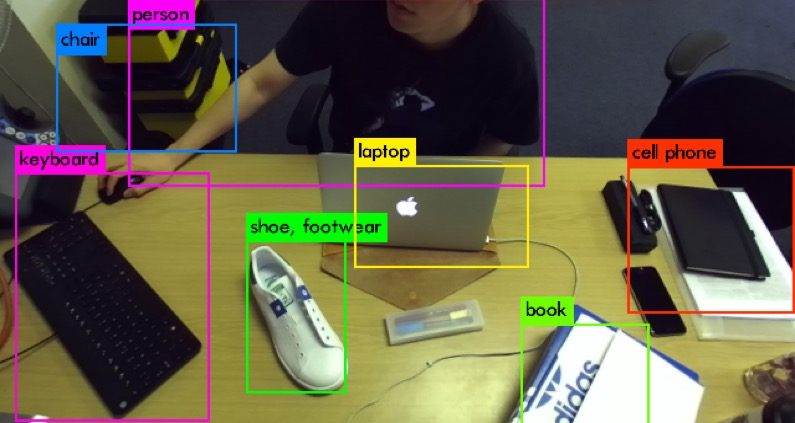
\includegraphics[width = 0.45\columnwidth]{TaR/yolot2.jpg}}
\caption{The examples of YOLO testing environments}
\end{figure}

Once YOLO detects a shoe, the following two situations will occur. When the shoe is vertically placed, the algorithm should publish the required four adjustment locations ($adr$, $adrr$, $adl$, and $adll$) to $TF$. If the shoe is in a good orientation, the 2D pixel coordinate of centroid of the shoe hole is supposed to be reported. Following tests will examine whether my approach can correctly classify the two situations and return the accurate results under the condition that YOLO can correctly detect the shoe.

\begin{table}[H]
\centering
\begin{tabular}{||c||c|c||}
\hline
 & Average execution time & Success rate \\ \hline \hline
Return adjustment locations & 0.01s & 20/20 \\ \hline
Return centroid coordinate & 0.046s & 30/30 \\ \hline
\end{tabular}
\caption{The testing results of situation classification}
\label{locationtest}
\end{table}

In the following experiment, I place the shoe vertically on the workbench for 20 times, and non-vertically for 30 times. Table \ref{locationtest} shows that my approach is able to classify the different situation with 100\% accuracy. Moreover, in most cases, the centroid location can be computed with high precision, as proved in Figure \ref{centroidresult}. 

\begin{figure}[H]
\centering
\subfigure[Correct]{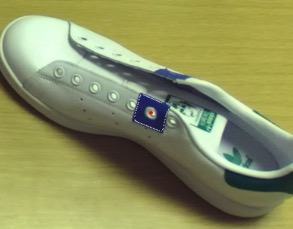
\includegraphics[height=3cm,keepaspectratio]{TaR/1.jpg}}
\subfigure[Correct]{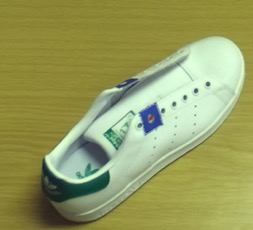
\includegraphics[height=3cm,keepaspectratio]{TaR/3.jpg}}
\subfigure[Correct]{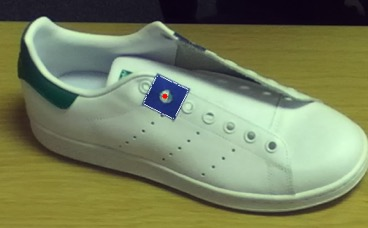
\includegraphics[height=3cm,keepaspectratio]{TaR/4.jpg}}
\subfigure[Correct]{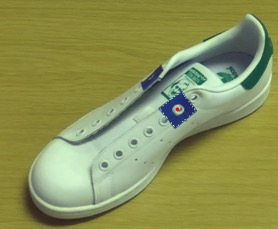
\includegraphics[height=3cm,keepaspectratio]{TaR/2.jpg}}
\subfigure[Correct]{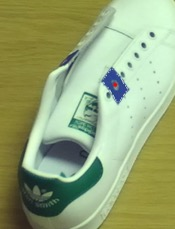
\includegraphics[height=3cm,keepaspectratio]{TaR/5.jpg}}
\subfigure[Small offset]{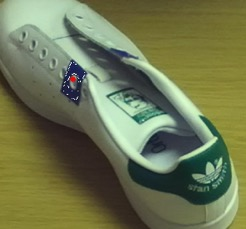
\includegraphics[height=3cm,keepaspectratio]{TaR/6.jpg}}
\caption{The examples of the computed 2D pixel position of the shoe hole. The contour is drawn in white, the centroid is marked in red.}
\label{centroidresult}
\end{figure}

Figure \ref{centroidresult} (f) is when the maximum error occurs. It can be discovered that there is a small offset between the red dot and the geometric center of shoe hole, which is considered to be acceptable.

\section{Shoe Pose Adjustment}
This section is to assess the performance of real shoe pose adjustment. Providing with four adjustment locations ($adr$, $adrr$, $adl$, and $adll$), YuMi will use both of its arms to adjust the orientation of the shoe accordingly. This feature was tested 20 times and the results are shown in Table \ref{adjusttest}.

\begin{table}[H]
\centering
\begin{tabular}{||c||c|c||}
\hline
 & Average execution time & Success rate \\ \hline \hline
Shoe pose adjustment & 33s & 19/20 \\ \hline
\end{tabular}
\caption{The testing results of situation classification}
\label{adjusttest}
\end{table}

The execution time is measured from \ref{realadjust} (a) to \ref{realadjust} (e), including total 5 movements. In 19 runs, YuMi finishes its job without failures. Only one adjustment fails: after YuMi adjusting the orientation of the shoe, both arms tried to return to Home pose, which is the motion after \ref{realadjust} (e). At this time, the left arm of YuMi collided with the heel-cap of the shoe because the height of end-effector is relatively low. The robot then stopped operation due to this detected collision. After I modifying the height settings at \ref{realadjust} (e), this problem was resolved and did not happen in later tests.


\section{Insertion and Pulling of The Shoelace}
So far, the accuracy of YuMi's approaching pose for shoelace insertion still depends on two factors: the accuracy of estimation of shoe hole orientation, and the offset adjustment. Together with my motion planning algorithm, the real shoe insertion tests were carried out 30 times based on the condition that the 2D pixel centroid of the shoe hole and its contour area are correctly computed. It was mentioned in the Requirement Capture Chapter that shoelace were assumed to be in YuMi gripper at the beginning. Therefore, in this experiment, I manually put the shoelace in the gripper and align their directions at initial stage (Figure \ref{putexample} (a)).

This experiment is divided into three levels: pass the shoe hole with $2.5mm$ radius, pass the shoe hole with $4.0mm$ radius, and pass the shoe hole with $7.5mm$ radius. The results are shown in Table \ref{insert}, where the execution time is recorded between Figure \ref{putexample} (a) and Figure \ref{putexample} (e), a total of three actions. 

\begin{table}[H]
\centering
\resizebox{\columnwidth}{!}{
\begin{tabular}{||c||c|c|c|c||}
\hline
 & \begin{tabular}[c]{@{}c@{}}Average \\ execution time\end{tabular} & \begin{tabular}[c]{@{}c@{}}Success rate \\ ($7.5mm$)\end{tabular} & \begin{tabular}[c]{@{}c@{}}Success rate \\ ($4.0mm$)\end{tabular}  & \begin{tabular}[c]{@{}c@{}}Success rate \\ ($2.5mm$)\end{tabular} \\ \hline \hline
Shoelace insertion & 9.65s & 30/30 & 25/30 & 12/30 \\ \hline
\end{tabular}
}
\caption{The testing results of shoelace insertion}
\label{insert}
\end{table}

It can be seen that the insertion success rate reach 100\% for relatively large hole, with $7.5mm$ radius. For normal $4mm$ radius shoe hole, YuMi successfully completed its job for 25 times out of 30 runs. For the 5 failure cases, two are because the orientation of shoelace was not perfectly aligned with the gripper, when I manually put it. It resulted in the end point of the gripper touched the hole but the shoelace failed to pass through. One failure is because Yumi's gripper came loose as it rotated. The final two turnovers are due to inaccurate computation of pose $shoe_hole$, when the shoe was placed in a relative bad angle.

As for $2.5mm$ shoe hole, there is more than half runs failed. Considering the diameter of the shoelace I used is approximately $2mm$, the movement must be extremely accurate to complete hole with this size. It shows that my algorithm still has room to improve, which will be further discussed in Future Work Chapter.

The shoelace grabbing test is based on the same condition as for shoelace insertion. In addition, I manually passed the shoelace along the normal vector direction of the hole. This experiment was carried out 20 times, whose operation time is between \ref{pickexample} (a) and \ref{pickexample} (e), a total of three movements. 

\begin{table}[H]
\centering
\begin{tabular}{||c||c|c||}
\hline
 & Average execution time & Success rate \\ \hline \hline
Shoelace grabbing & 9.35s & 17/20 \\ \hline
\end{tabular}
\caption{The testing results of shoelace grabbing}
\label{pull}
\end{table}

Table \ref{pull} are the testing results. In the three turnovers, two are because the yaw rotation of end-effector was not perfectly parallel to the tongue, which results in slight collision between the finger and the lace guard. The final failure is because the black finger (the one 3D printed) suddenly broke when it tried to close and grab the shoelace. That finger was 3D printed again and reattached to YuMi.

\section{Integrated System Performance}
After testing every individual functionality, the performance of the integrated system was then examined. This experiment starts from randomly placing the shoe on the workbench, YuMi should adjust the shoe pose if necessary. Once the shoe is in a good position, the shoelace was manually put in and aligned with the YuMi gripper. After that, YuMi are supposed to pass it into the shoe hole and pull it out. The shoe hole used in this experiment has $4mm$ radius.

\begin{table}[H]
\centering
\resizebox{\columnwidth}{!}{
\begin{tabular}{||c||c|c|c|c|c||}
\hline
 \begin{tabular}[c]{@{}c@{}}Placement of \\ the shoe\end{tabular} & \begin{tabular}[c]{@{}c@{}}Average \\ execution time\end{tabular} & \begin{tabular}[c]{@{}c@{}}Success rate \\ for detection\end{tabular} & \begin{tabular}[c]{@{}c@{}}Success rate \\ for adjustment\end{tabular} & \begin{tabular}[c]{@{}c@{}}Success rate \\ for insertion\end{tabular} & \begin{tabular}[c]{@{}c@{}}Success rate \\ for pulling\end{tabular}
 \\ \hline \hline
Bad position & 116s & 20/20 & 19/20 & 17/19 & 16/17 \\ \hline
Good position & 60s & 20/20 & -- & 17/20 & 15/17 \\ \hline
\end{tabular}
}
\caption{The testing results of integrated system}
\label{integratedtest}
\end{table}

Table \ref{integratedtest} illustrates the final results. In all 40 runs, the detection algorithm can successfully detect the shoe and return either the location of the shoe hole or the adjustment points. When the initial position of the shoe is not ideal, the system succeeded to adjust the shoe pose for 19 times out of 20. That one failure is because both grippers were relatively close to the vertical middle of the shoe during the adjustment, which resulted in when they both moved towards the horizontal middle, YuMi suddenly entered the motion supervision mode. After that, I modified my algorithm to let the adjustment points ($adr$, $adl$) more separate to each other, based on the condition that the orientation of the shoes can still be adjusted. 

There are 5 failures for shoelace insertion, 4 of which are due to the inaccurate estimation of $shoe\_hole$ location. The maximum error between the predicted and actual location is $3mm$, which again proves the system can successfully handle $7.5mm$ radius shoe hole. The other failure is because motion planning algorithm failed to provide a valid path, YuMi did not move but return to Cal pose directly. 

As for shoelace pulling section, there are 3 turnovers. One is because the shoelace slipped out of the shoe hole after it being successfully inserted. For the other two failures, the head of the shoelace was dragged down by its weight, so that the gripper missed it. These problems can be tackled by keeping the right arm at insertion pose while letting the left arm to grab the shoelace, which will be implemented ............

\begin{figure}[H]
\centering
\subfigure[Bad shoe position]{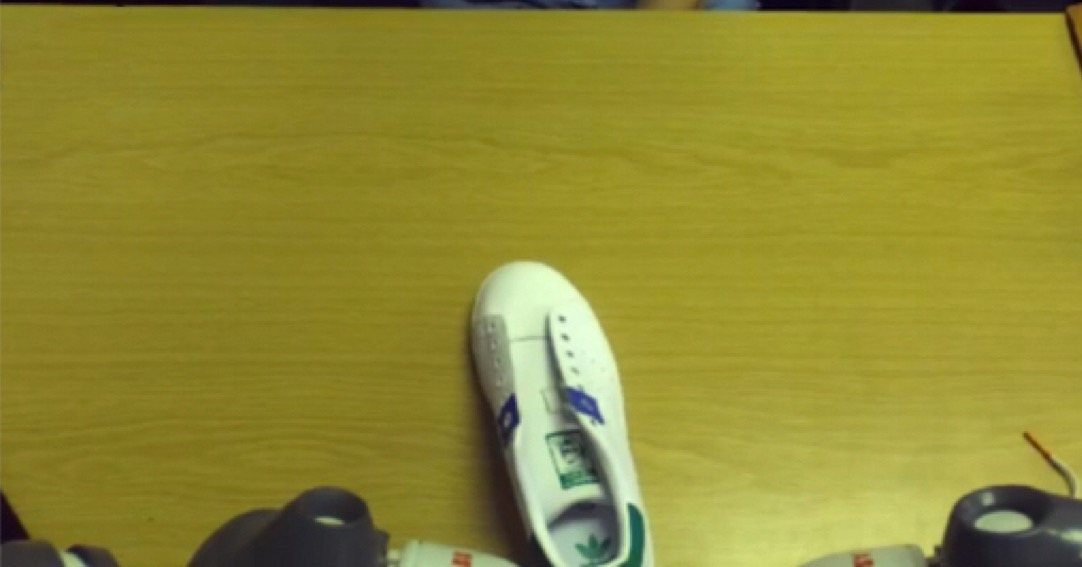
\includegraphics[width = 0.24\columnwidth]{TaR/t1.jpg}}
\subfigure[Pre-adjust]{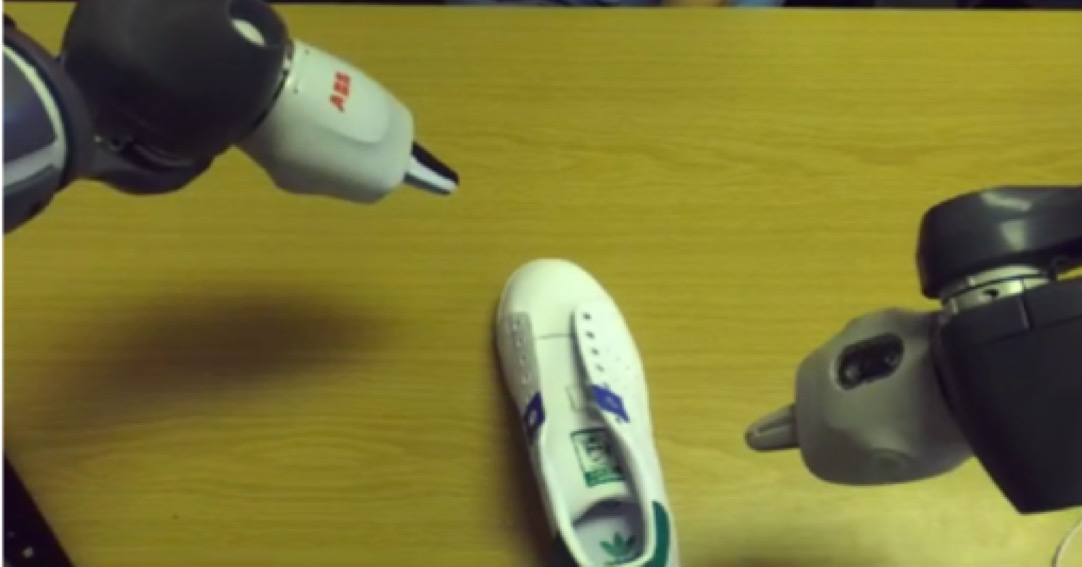
\includegraphics[width = 0.24\columnwidth]{TaR/t2.jpg}}
\subfigure[Pre-adjust]{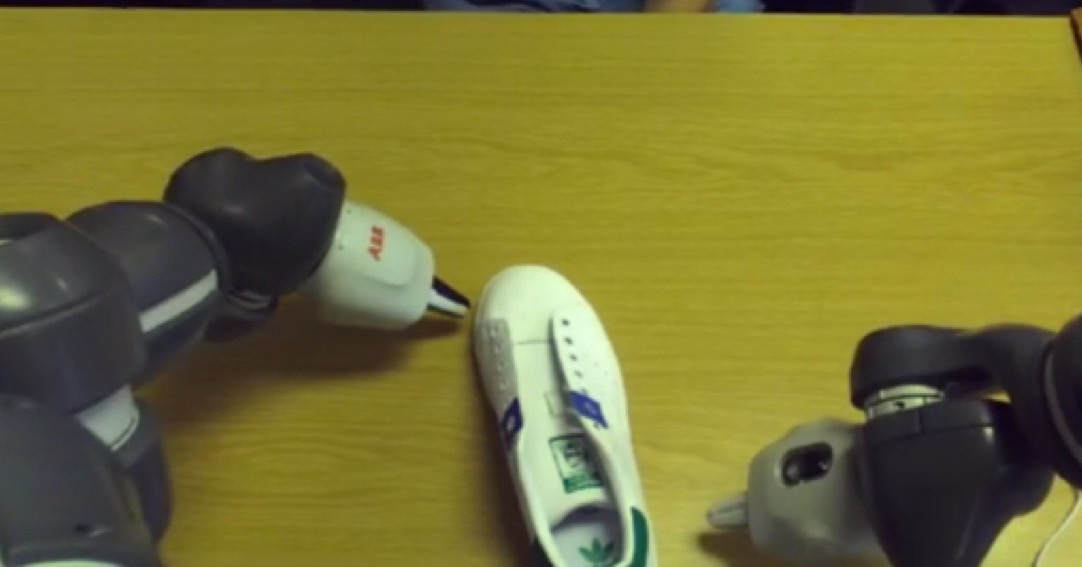
\includegraphics[width = 0.24\columnwidth]{TaR/t3.jpg}}
\subfigure[Adjust]{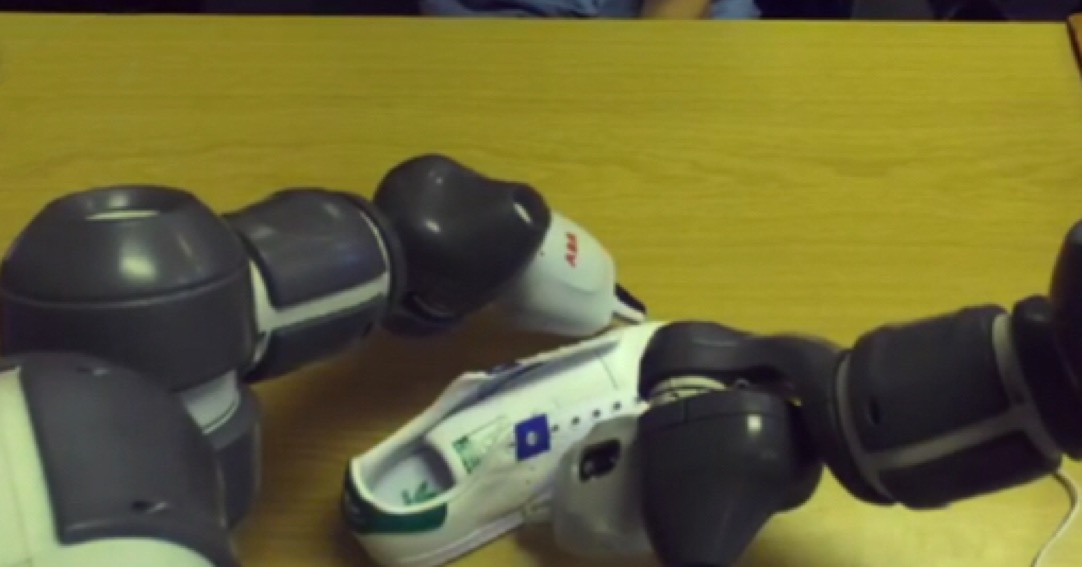
\includegraphics[width = 0.24\columnwidth]{TaR/t4.jpg}}

\subfigure[Post-adjust]{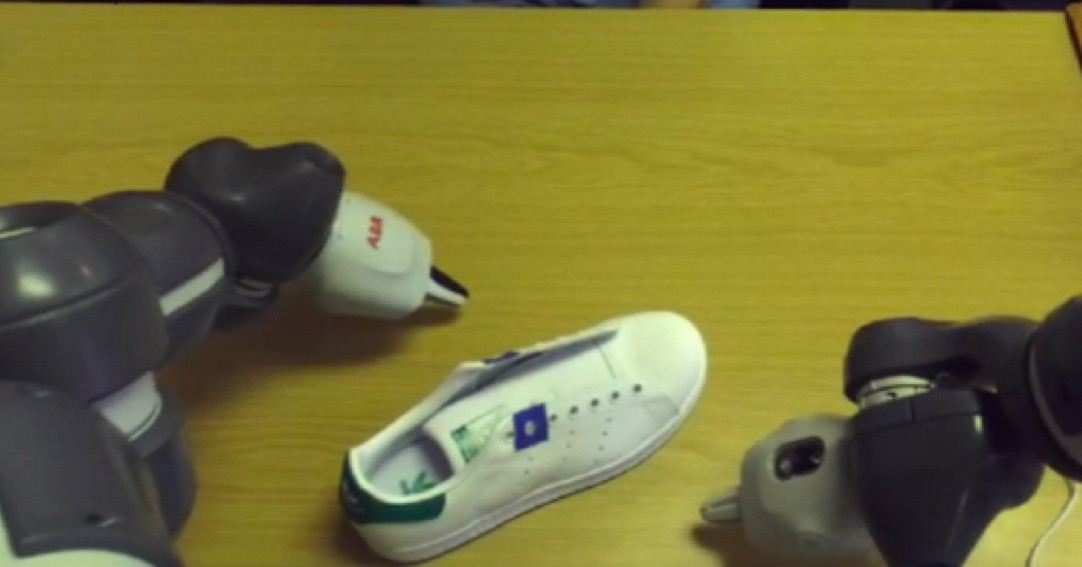
\includegraphics[width = 0.24\columnwidth]{TaR/t5.jpg}}
\subfigure[Post-adjust]{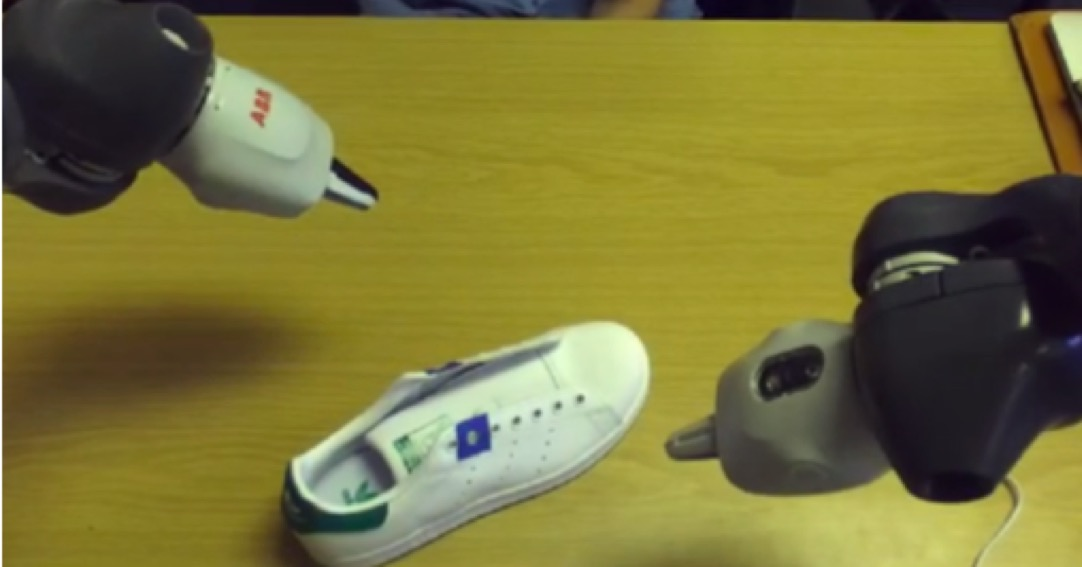
\includegraphics[width = 0.24\columnwidth]{TaR/t6.jpg}}
\subfigure[Home pose]{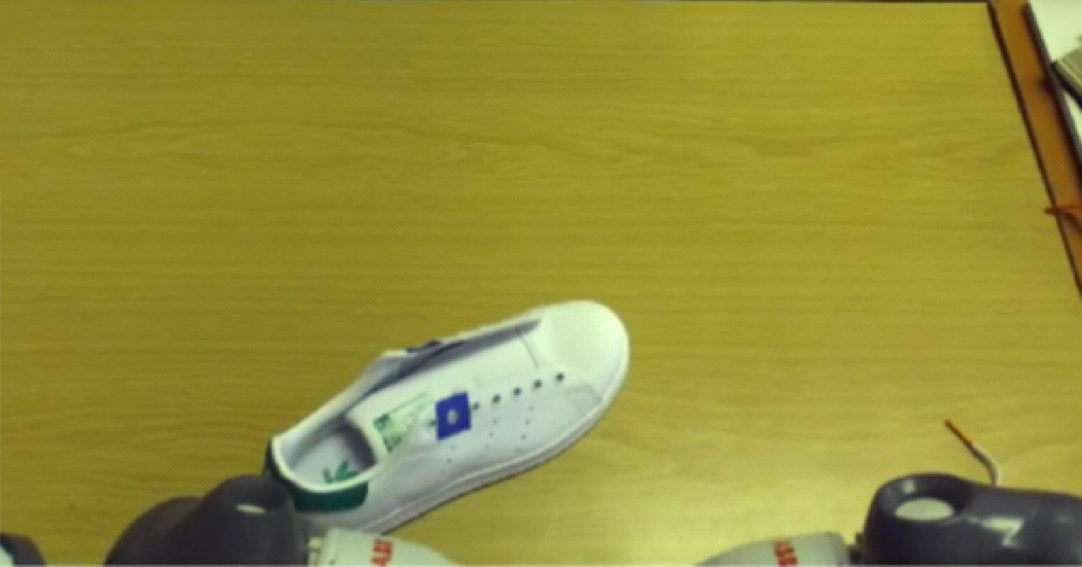
\includegraphics[width = 0.24\columnwidth]{TaR/t7.jpg}}
\subfigure[Attach shoelace]{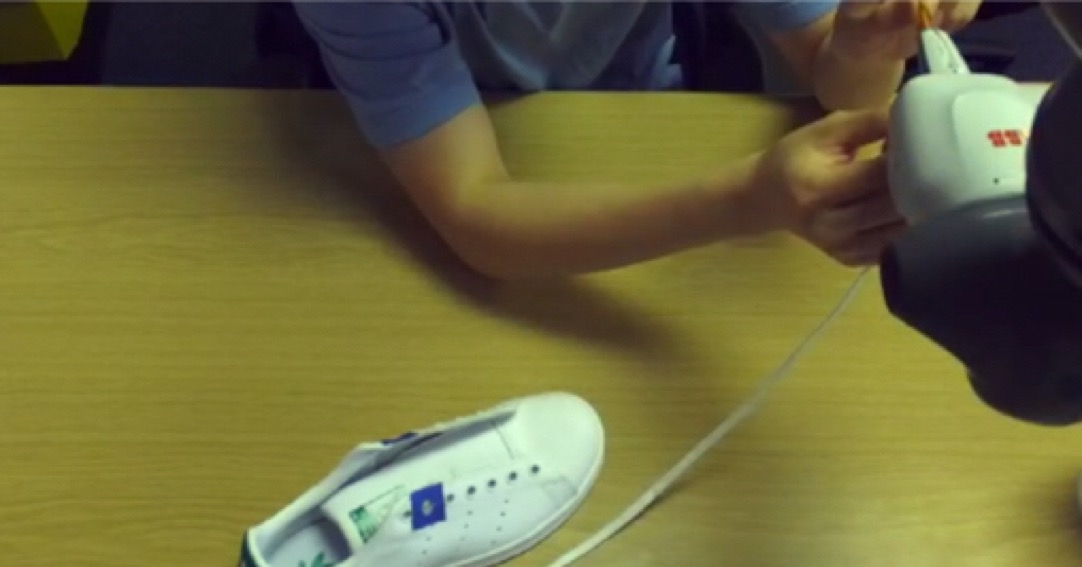
\includegraphics[width = 0.24\columnwidth]{TaR/t8.jpg}}

\subfigure[Pre-put]{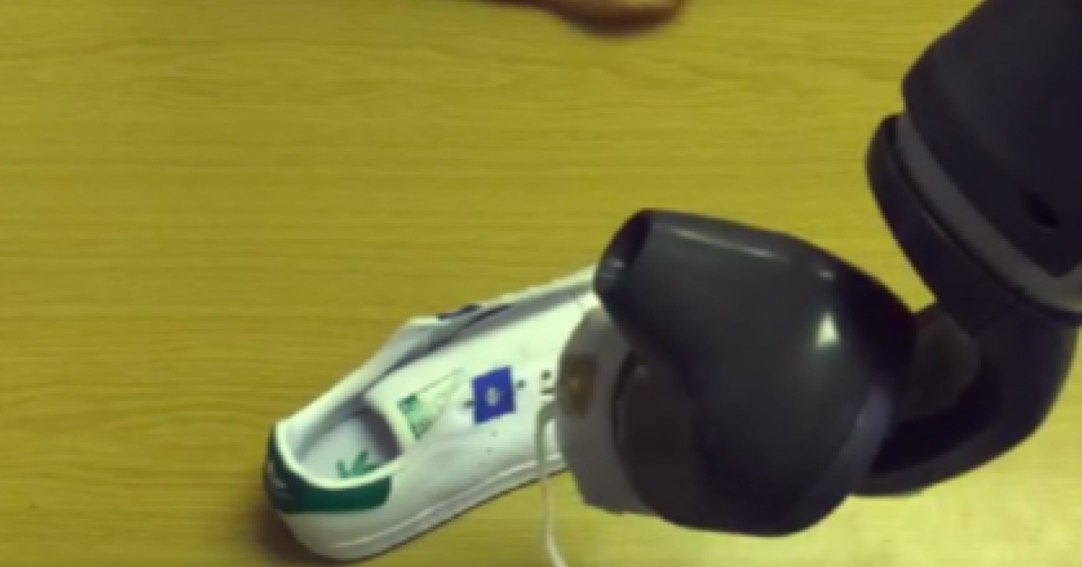
\includegraphics[width = 0.24\columnwidth]{TaR/t9.jpg}}
\subfigure[Insertion]{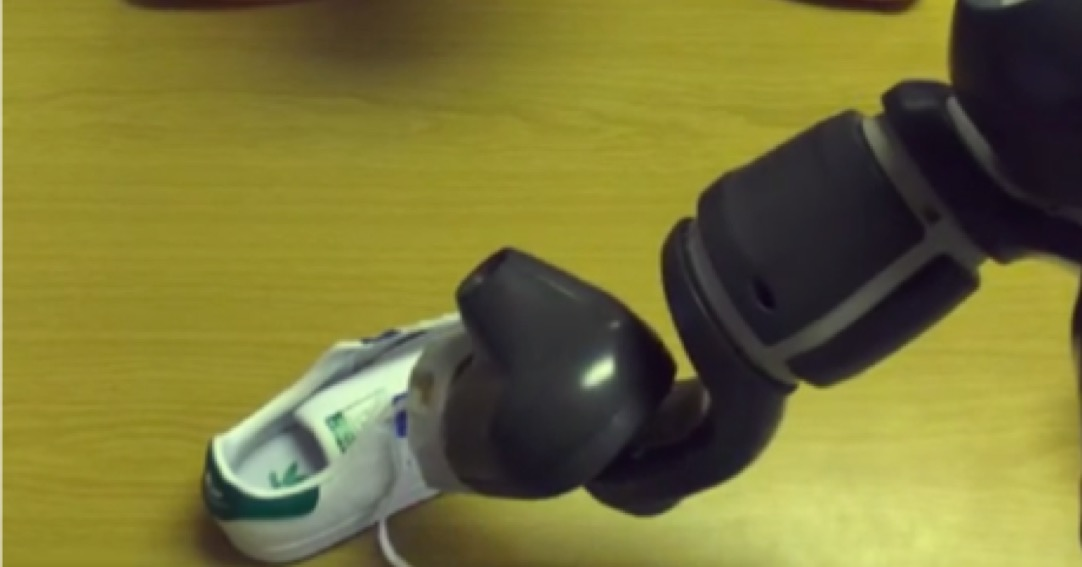
\includegraphics[width = 0.24\columnwidth]{TaR/t16.jpg}}
\subfigure[Pose-put]{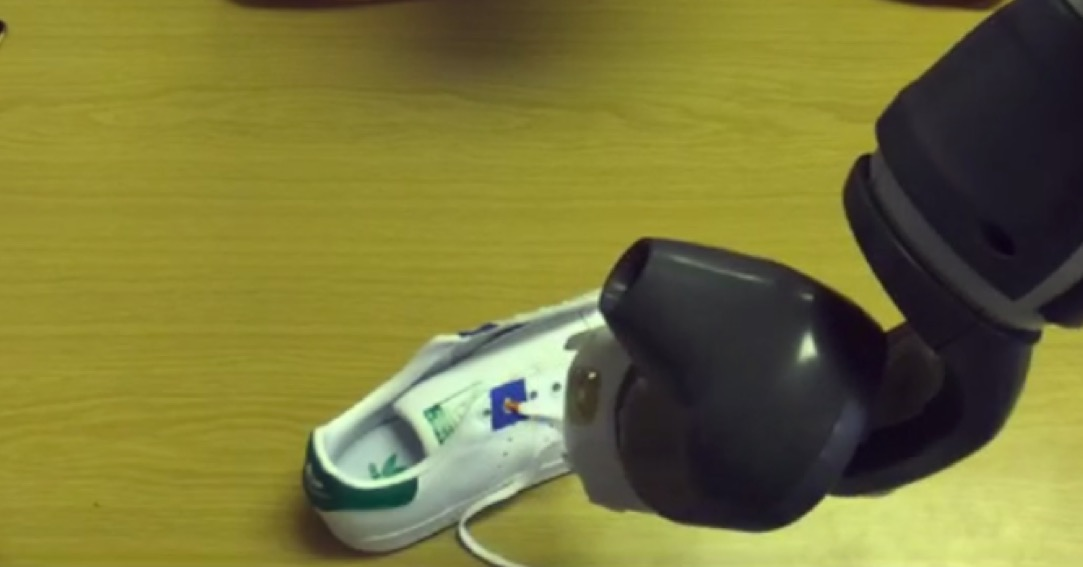
\includegraphics[width = 0.24\columnwidth]{TaR/t10.jpg}}
\subfigure[Home pose]{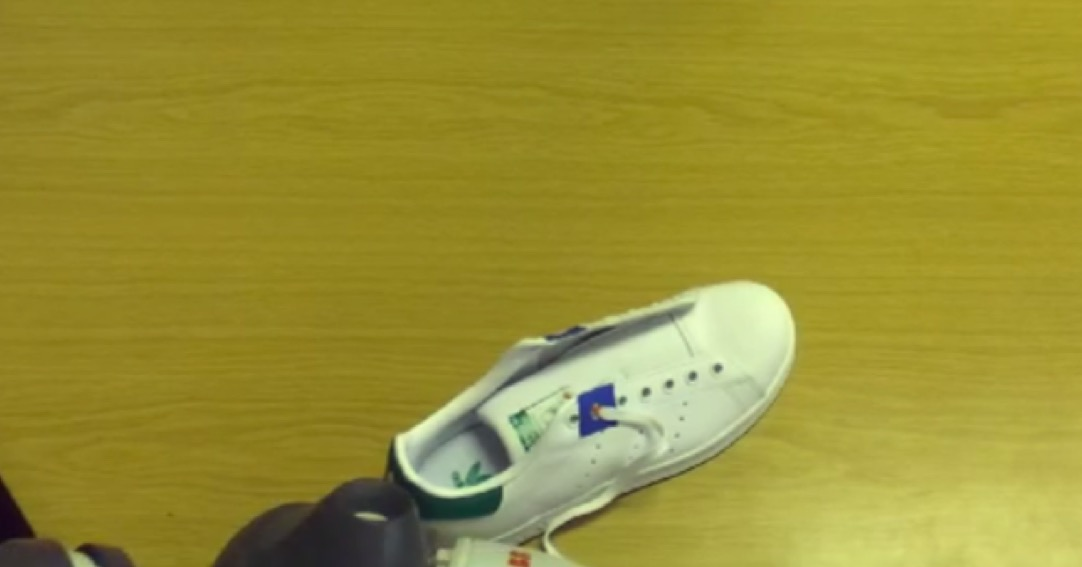
\includegraphics[width = 0.24\columnwidth]{TaR/t11.jpg}}

\subfigure[Pre-grabbing]{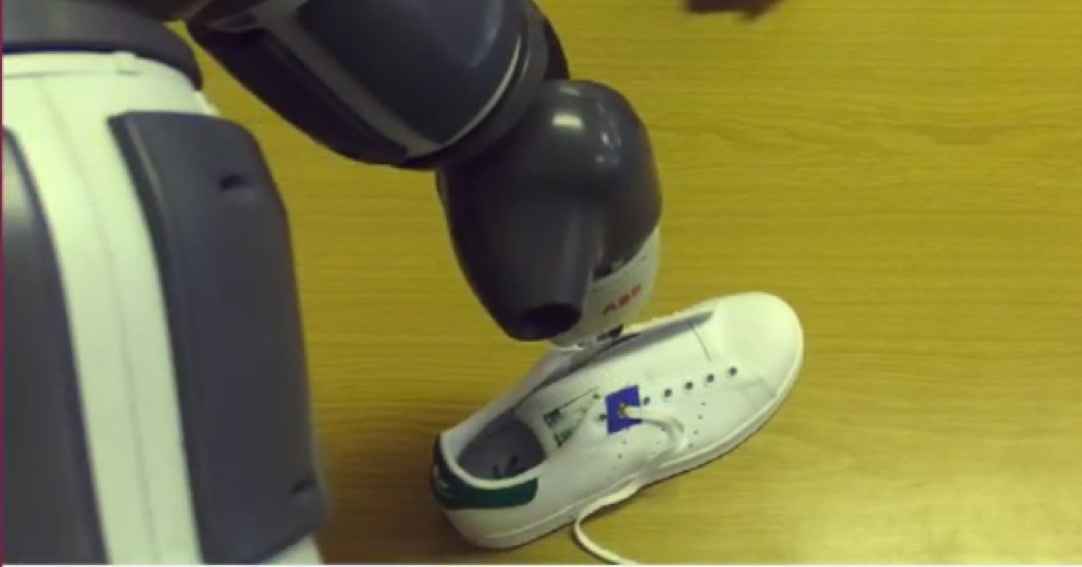
\includegraphics[width = 0.24\columnwidth]{TaR/t12.jpg}}
\subfigure[Grabbing]{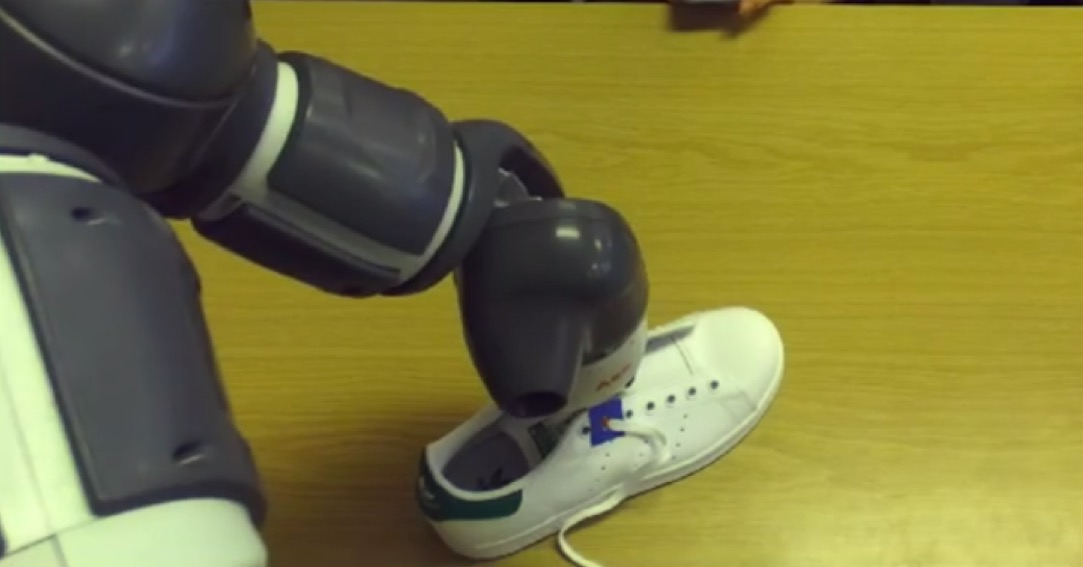
\includegraphics[width = 0.24\columnwidth]{TaR/t13.jpg}}
\subfigure[Post-grabbing]{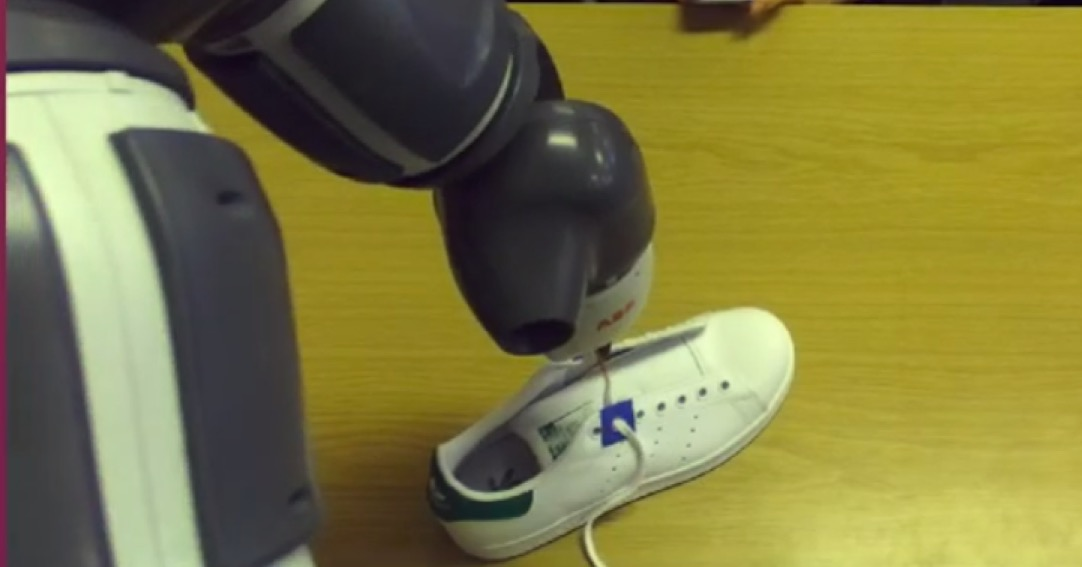
\includegraphics[width = 0.24\columnwidth]{TaR/t14.jpg}}
\subfigure[Home pose]{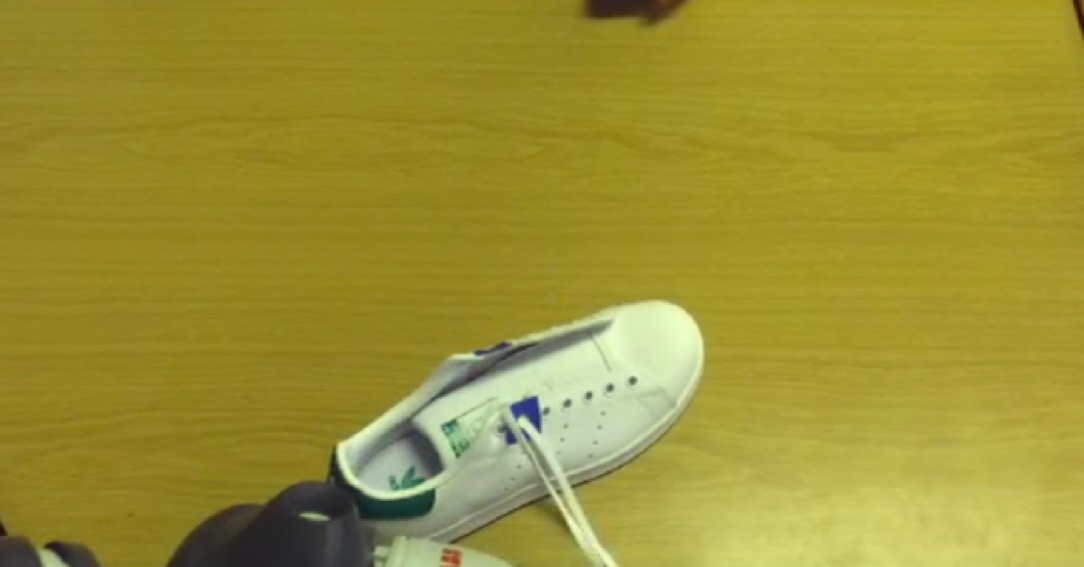
\includegraphics[width = 0.24\columnwidth]{TaR/t15.jpg}}
\caption{Example of the manipulation process: adjusting shoe pose, insert shoelace, pull shoelace out}
\label{integratedtestfig}
\end{figure}

Figure \ref{integratedtestfig} shows a series of YuMi manipulation photos captured by the external camera ZED Mini. In this example the shoe pose has been successfully adjusted and the shoelace were inserted and pulled out.